\documentclass[10pt]{book}

%These tell TeX which packages to use.
\usepackage{array,epsfig}
\usepackage{amsmath}
\usepackage{amsfonts}
\usepackage{amssymb}
\usepackage{amsxtra}
\usepackage{amsthm}
\usepackage{mathrsfs}
\usepackage{color}
\usepackage{enumitem}
%\usepackage{mdframed}
\usepackage[most]{tcolorbox}
\usepackage{pgfplots}
\pgfplotsset{compat=1.6}

\pgfplotsset{soldot/.style={color=black,only marks,mark=*}} \pgfplotsset{holdot/.style={color=black,fill=white,only marks,mark=*}}

%Here I define some theorem styles and shortcut commands for symbols I use often
\theoremstyle{definition}
\newtheorem{defn}{Definition}
\newtheorem{thm}{Theorem}
\newtheorem{cor}{Corollary}
\newtheorem*{rmk}{Remark}
\newtheorem{lem}{Lemma}
\newtheorem*{joke}{Joke}
\newtheorem{ex}{Example}
\newtheorem*{soln}{Solution}
\newtheorem{prop}{Proposition}

\newcommand{\lra}{\longrightarrow}
\newcommand{\ra}{\rightarrow}
\newcommand{\surj}{\twoheadrightarrow}
\newcommand{\graph}{\mathrm{graph}}
\newcommand{\bb}[1]{\mathbb{#1}}
\newcommand{\Z}{\bb{Z}}
\newcommand{\Q}{\bb{Q}}
\newcommand{\R}{\bb{R}}
\newcommand{\C}{\bb{C}}
\newcommand{\N}{\bb{N}}
\newcommand{\M}{\mathbf{M}}
\newcommand{\m}{\mathbf{m}}
\newcommand{\MM}{\mathscr{M}}
\newcommand{\HH}{\mathscr{H}}
\newcommand{\Om}{\Omega}
\newcommand{\Ho}{\in\HH(\Om)}
\newcommand{\bd}{\partial}
\newcommand{\del}{\partial}
\newcommand{\bardel}{\overline\partial}
\newcommand{\textdf}[1]{\textbf{\textsf{#1}}\index{#1}}
\newcommand{\img}{\mathrm{img}}
\newcommand{\ip}[2]{\left\langle{#1},{#2}\right\rangle}
\newcommand{\inter}[1]{\mathrm{int}{#1}}
\newcommand{\exter}[1]{\mathrm{ext}{#1}}
\newcommand{\cl}[1]{\mathrm{cl}{#1}}
\newcommand{\ds}{\displaystyle}
\newcommand{\vol}{\mathrm{vol}}
\newcommand{\cnt}{\mathrm{ct}}
\newcommand{\osc}{\mathrm{osc}}
\newcommand{\LL}{\mathbf{L}}
\newcommand{\UU}{\mathbf{U}}
\newcommand{\support}{\mathrm{support}}
\newcommand{\AND}{\;\wedge\;}
\newcommand{\OR}{\;\vee\;}
\newcommand{\Oset}{\varnothing}
\newcommand{\st}{\ni}
\newcommand{\wh}{\widehat}
%Pagination stuff.
\setlength{\topmargin}{-0.75in}
\setlength{\oddsidemargin}{0in}
\setlength{\evensidemargin}{0in}
\setlength{\textheight}{9.in}
\setlength{\textwidth}{6.5in}
\pagestyle{empty}
\begin{document}
\begin{flushleft}
Name:\underline{\hspace{13cm}}Date:\underline{\hspace{2cm}}
\end{flushleft}
\begin{center}
{\Large Math 1041-012 \hspace{0.5cm} Section 2.8: Derivative as a Function}
\end{center}
%\vspace{0.2 cm}
\begin{tcolorbox}
\subsection*{Definition}
The derivative function $f'(x)$ is given by
\[
f'(x)=\lim_{h\rightarrow 0}\frac{f(x+h)-f(x)}{h}
\]
\end{tcolorbox}
\subsection*{Example 1: Find $f'(x)$}
\begin{itemize}
    \item[(a)] If $f(x)=x^3-x$ find a formula for $f'(x)$.\vspace{5cm}
    \item[(b)] If $f(x)=\sqrt{x}$ find the derivative.\vspace{5cm}
    \item[(c)] Find $f'(x)$ if $\displaystyle f(x)=\frac{1-x}{2+x}$
\end{itemize}
\raggedbottom
\clearpage
\begin{tcolorbox}
\subsection*{Is a function always differentiable at a number?} not if...
\begin{itemize}
    \item there are discontinuites,
    \item kinks, cusps in graph,
    \item vertical tangents,
\end{itemize}
\subsubsection*{Definition}
A function $f$ is \textbf{differentiable} at a number ``$a$'' if $f'(a)$ exists. It is differentiable on an open interval $(a,b)$ if it is diffentiable at every number in the interval.\\ \\
Note: If $f$ is differentiable at $a$, then it is continuous at $a$. (is the other direction true??)
\end{tcolorbox}
\begin{figure}[h!]
    \centering
    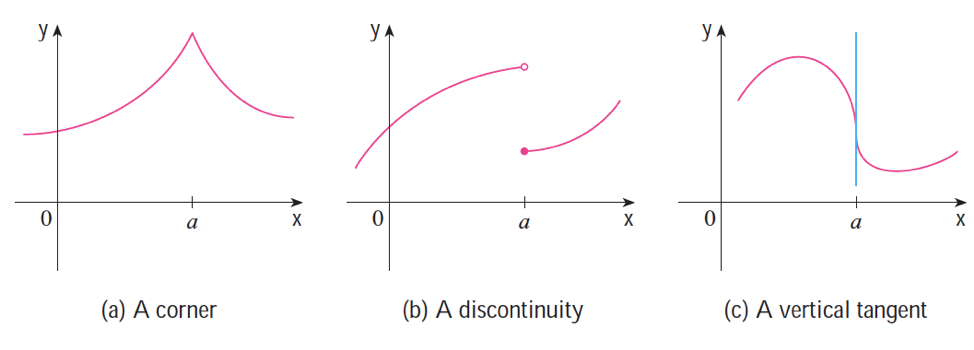
\includegraphics[scale=0.65]{fig1.png}
\end{figure}
\subsection*{Example 2}
Where is the function $f(x)=|x|$ differentiable?
\raggedbottom
\clearpage
\begin{tcolorbox}
\subsection*{Higher Derivatives}
\begin{itemize}
    \item $f''(x)$ means find the second derivative. This means find the derivative of the derivative. Can also be written as:
    \item $f'''(x)$ means find the third derivative....
\end{itemize}
\end{tcolorbox}
\subsection*{Example 3}
Given $y=f(x)=x^3-x$, find $\displaystyle\frac{dy}{dx}, \frac{d^2y}{dx^2},\frac{d^3y}{dx^3}$.
\end{document}